% What is model based control?
% Video to text vs. Video language models?
\chapter{Learning from Videos - Data Modality and Challenges}

Videos are a challenging data modality, as you have seen in Section~\ref{sec:ChallengesOfVideoData}. This section addresses the two key questions for \ac{LfV} research:
\begin{enumerate}
    \item How to extract relevant knowledge from internet video?
    % \item How to apply video-extracted knowledge to robotics?
    \item How to apply video-extracted knowledge to robotic systems for policy learning and control?
\end{enumerate}
We first review different approaches for extracting foundational knowledge from internet video, including video encoders, video prediction models, and video-to-text models. We then discuss methods for transferring video-extracted knowledge to robotics, addressing challenges such as missing action labels and distribution shift. 

% it is high-dimensional, noisy, and poorly labelled. Second, video lacks information critical to robotics, including action labels and low-level force and proprioceptive information. Moreover, there may be various distribution shifts between internet video and the robot domain.


\section{Extracting Foundational Knowledge from Internet Video} 
\label{sec:ExtractingFoundationalKnowledgeFromInternetVideo}

% The Answer to the first question of how to extract relevant knowledge from internet video is may be using techniques and datasets inspired by video foundation Models (FMs).

Recent progress in \textbf{Video \acp{FM}} provides a promising direction for addressing the first answer: How to extract robotic relevant knowledge from internet video. Video \acp{FM} are large-scale deep learning models trained on massive internet video datasets. Through large-scale training, these models learn general visual and temporal representations that capture semantics, motion dynamics, physical interactions and behavioral patterns. As a result, they can extract foundational knowledge that is transferable across a wide range of downstream tasks, including robotics applications \cite{Madan2024FoundationMF}.

\begin{samepage}
McCarthy et al. \cite{McCarthy_2025} says, Video \acp{FM} can be highly applicable for the following \ac{LfV} use-cases, see Figure \ref{fig:VideoFoundationModellingForLfV}:
\begin{itemize}
    \item \texttt{Finetune Pretrained Video \acp{FM}:} 
    One important application of Video \acp{FM} is the transfer of pretrained models to robotics tasks. For example, a video prediction model trained on internet video data may be adapted or fine-tuned into a robot dynamics model, allowing the robot to leverage the broad gathered knowledge about object motion and environmental dynamics from the pretrained Video \acp{FM} \cite{Yang2023LearningIR, rt22023arxiv, Ahn2022DoAI, Kim2024OpenVLAAO}. 
    
    \item \texttt{Leveraging Techniques and Datasets Inspired by Video \acp{FM}:}
    In addition, techniques developed for video foundation models can be integrated into robot learning pipelines and can lead to better extraction of representations and knowledge. This, in turn, can lead to improved generalization and task understanding. For instance, a Robot \ac{FM} can be directly trained by combining robot data with large-scale video inspired by video \acp{FM} techniques \cite{Team2024OctoAO, rt12022arxiv}.
\end{itemize}
\end{samepage}

\begin{figure}
	\centering
	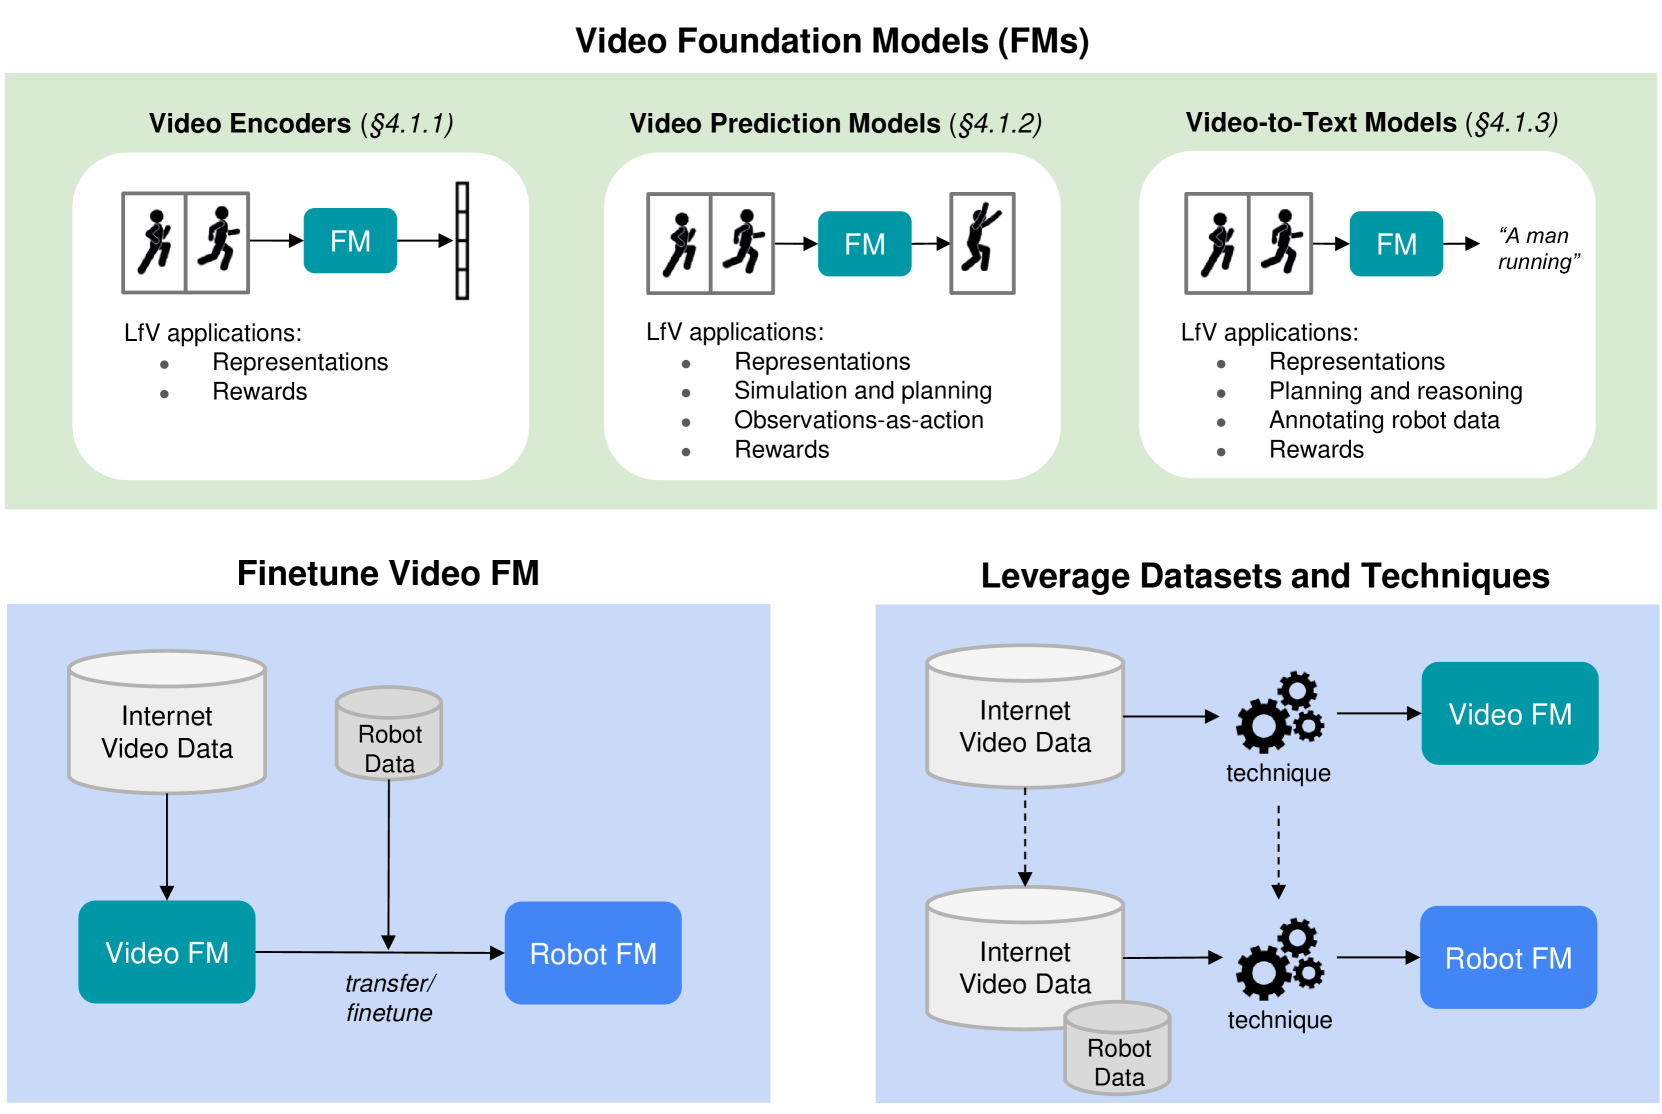
\includegraphics[width=1.0\linewidth]{./chapter5/media/VideoFoundationModellingForLfV}
	\caption[Video Foundation Modelling for LfV]{Video foundation modelling for Learning from Videos. Image source: \cite{McCarthy_2025}.}
	\label{fig:VideoFoundationModellingForLfV}
\end{figure}

% Furthermore, these models can serve as strong initialization policies for \ac{RL}. A common strategy is to first pretrain the model using supervised sequence prediction on large-scale multimodal datasets, and subsequently fine-tune the policy using \ac{RL} with task-specific rewards. This often improves sample efficiency and generalization compared to training \ac{RL} policies from scratch.
% Even when the action prediction head is discarded, the learned encoder can still provide transferable cross-modal representations for downstream robotic tasks. 


\subsection{Video Encoders}
\label{sec:VideoEncoder}
Foundational video encoders are capable of extracting rich and robust representations from raw video observations:
\begin{equation}
    p(z \mid \tau)
\end{equation}
Given a video clip $\tau$, the encoder maps the visual input into a latent representation $z$, which captures semantic and temporal information relevant for downstream robotic tasks.

\paragraph{Relevance for Robotics.}
In robotic \ac{IL}, pretrained video encoders are commonly used in two ways \cite{McCarthy_2025}:
\begin{itemize}
    \item \texttt{Representation Learning:}
    Pretrained video encoders can be transferred to robotic learning frameworks and further fine-tuned on robot-specific data for downstream tasks such as policy learning or an \ac{RL} \ac{KM}. The learned latent representations provide compact and informative features that improve generalization and sample efficiency, by allowing the model to learn task-specific features while still leveraging the general knowledge captured from internet video
    % ToDo: , see Section~\ref{} and maybe some references.
    
    \item \texttt{Reward Learning:} 
    Frozen video representations can also be used to define reward functions for robotic agents \cite{Nair2022R3MAU, Sontakke2023RoboCLIPOD, Fan2022MineDojoBO}. By comparing the latent representations of demonstrations and robot executions, the system can measure behavioral similarity without requiring manually engineered reward signals. This approach enables the robot to learn from video demonstrations by optimizing its behavior to match the latent representations of successful demonstrations, thus facilitating \ac{IL} and skill acquisition.
    % ToDo: , see Section~\ref{}.
\end{itemize}

\subsubsection{Methods}
\paragraph{Video Representation Learning}
Video representation learning aims to learn meaningful latent representations from raw video data. These representations capture semantic, spatial and temporal information that can be used for various downstream tasks \cite{McCarthy_2025}.

Let
\begin{itemize}
    \item $X$ denote a video clip
    \item $\bar X$ denote a video clip paired with some corresponding labels (bounding boxes and object masks \cite{Ding2023MOSEAN}) and data modalities (language annotations \cite{Grauman2021Ego4DAT}, meta-data \cite{ChantrySchiappa2022SelfSupervisedLF})
    \item $Y$ denote a learning objective, derived from $\bar X$
\end{itemize}
\texttt{Learning Goal During Training:} predict $Y$ from $X$.
Or in other words, learn a video encoder $p(z|X)$ that maps the video clip $X$ to a latent representation $z$ that can be used to predict $Y$: $X \xrightarrow{p(z|X)} z \rightarrow Y$ \cite{McCarthy_2025}.
% The objective of the video encoder $p(z|X)$ is then to learn representations $z$ that enable the prediction or alignment of $Y$ from the input video $X$.
% During training, the objective is to learn representations $z$ that enable the prediction or alignment of $Y$ from the input video $X$.
Basic techniques for learning $Y$ include:
\begin{itemize}
    \item \textbf{Prediction-Based Objectives}: The target $Y$, which is derived from the annotated video clip $\bar X$, may correspond to future video frames, masked regions, motion information, or other supervision signals. For example, in video prediction tasks, the model predicts the next frame $x_{t+1}$ from the raw previous observations $x_{\leq t}$ \cite{Gao2022SimVPSY, Jang2024VisualRL}. 
    % The Encoder is optimized using a prediction loss that encourages the learned representation to capture temporal structure and motion dynamics in video sequences.
    % The encoder is optimized using a prediction loss of the form
    % \begin{equation}
    % \mathcal{L}_{\text{pred}} = \| \hat{Y} - Y \|^2
    % \end{equation}
    % where $\hat{Y}$ denotes the predicted target. 
    % Such objectives encourage the learned representation to capture temporal structure and motion dynamics in video sequences.

    \item \textbf{Joint-Embedding Objectives}: Joint-embedding approaches \cite{Oord2018RepresentationLW, Xian2023TowardsGR, bardes2023v} first map both the video input $X$ and the known target $Y$ into a shared latent embedding space:
    \begin{equation}
    z_X = f(X),
    \qquad
    z_Y = g(Y)
    \end{equation}

    A loss function is then applied to align semantically similar embeddings: 
    \begin{equation}
    \mathcal{L}_{\text{pred}} = L_{\text{align}}(z_X, z_Y)
    \end{equation}
    Contrastive learning is one of the most widely used approaches in this setting \cite{ChantrySchiappa2022SelfSupervisedLF}. 
    % These approaches have become highly effective for learning transferable video representations from large-scale unlabeled video datasets.
\end{itemize}


\paragraph{State-of-the-Art Approaches}
Recent work has proposed scalable methods for learning rich spatio-temporal video representations. 
\textit{Video-Text Objectives:} Video-text objectives leverage language annotations to learn semantic representations from video data. Common approaches include:
\begin{itemize}
    \item \textbf{Video-Text Contrastive Learning:} This approaches learn to align video representations with corresponding text descriptions. By maximizing the similarity between video and text embeddings, the model captures semantic relationships between visual content and language \cite{Xu2021VideoCLIPCP, Zhao2024VideoPrismAF, Wang2023InternVidAL, Papalampidi2023ASR, Li2023UnmaskedTT}.
    
    \item \textbf{Video-Text Matching:} This methods train the model to determine whether a given video clip and text description correspond to each other. The model learns to distinguish between matching and non-matching pairs, which encourages it to capture relevant features for both modalities \cite{Li2023UnmaskedTT}.

    \item \textbf{Masked Language Modelling:} In this approaches, the model learns to predict masked words in a text description based on the corresponding video content. This encourages the model to learn contextual relationships between visual information and language \cite{Li2023UnmaskedTT}.

    % ToDo: steht als Video-to-text losses in McCarthy2025 --> ist das hier so richtig
    \item \textbf{Video-to-Text Generation:} This method trains the model to generate descriptive text based on video input. By learning to produce coherent and relevant descriptions, the model captures high-level semantic information from the video data \cite{Papalampidi2023ASR, Yan2022VideoCoCaVM}.
\end{itemize}


\textit{Auto-Encoding Approaches.} Auto-encoding approaches have also become highly effective for self-supervised video representation learning. Auto-encoding approaches learn video representations by reconstructing input data from compressed latent representations. Common approaches include:
\begin{itemize}
    \item \textbf{\ac{MAE}:} In this approach, parts of the video input are randomly masked, and the model is trained to reconstruct the missing regions from the visible observations. This encourages the encoder to learn meaningful spatial and temporal representations from incomplete video information \cite{Wang2023VideoMAEVS, Tong2022VideoMAEMA, Girdhar2022OmniMAESM}.
    % This method learns to reconstruct masked regions of video input, encouraging the model to capture meaningful spatio-temporal structure and context from incomplete observations.
    
    \item \textbf{\ac{VQ-AE}:} 
    In this approach, the encoder first extracts continuous latent features from the video input. 
    These features are then quantized by mapping them to the nearest vector in a finite set of learned codebook embeddings/vectors. 
    The decoder reconstructs the original video from these vector, encouraging the model to learn compact and semantically meaningful representations, due to the limited set of learned embeddings. 
    The underlying principle is similar to language modelling, where a finite vocabulary of discrete tokens is used to represent words, syllables or letters. Analogously, \ac{VQ-AE} learns a finite set of discrete visual tokens that capture recurring patterns in video data. These tokens may represent object appearances, motion patterns, textures, actions, or scene structures \cite{Bruce2024GenieGI, Villegas2022PhenakiVL, Yu2022MAGVITMG, Yan2021VideoGPTVG, Seo2022HARPAL}. 
    % By reusing a limited set of learned embeddings, the model can construct compact and semantically meaningful representations of complex visual observations.
\end{itemize}

\textit{Student-Teacher Distillation Approaches.} Student-teacher distillation approaches learn representations by transferring knowledge from a pretrained teacher network to a smaller student model \cite{Zhao2024VideoPrismAF, Wang2022MaskedVD, Li2023UnmaskedTT}. The student is trained to match the representations or predictions generated by the teacher model. This encourages the student network to learn robust and generalized video representations while often requiring fewer computational resources.

% \item \textbf{Student-Teacher Distillation:} These methods train a student network to match the representations of a pretrained teacher model, transferring knowledge and improving generalization.

\texttt{Joint-Embedding Predictive Architectures (JEPA)} learn representations by predicting high-level latent embeddings instead of reconstructing raw video pixels. Rather than modeling every visual detail, the model predicts semantic representations of future or masked observations in a shared embedding space. This approach improves robustness against the high-dimensionality and noise commonly present in video data while focusing on semantically relevant information \cite{bardes2023v}.
%  The learned representations can then be used for tasks such as action recognition, video classification, and robotic control.






\subsection{Video Prediction Models}
\label{sec:VideoPredictionModels}
Video prediction models aim to model the conditional distribution over future visual observations given past context \cite{McCarthy_2025}. The standard formulation is next-frame prediction:
\begin{equation}
p(o_{t+1} \mid o_{t-k:t})
\end{equation}
While more generally Video prediction models can be expressed as conditional video generation models:
\begin{equation}
    p(\tau \mid c)
\end{equation}
Where $\tau$ is a video sequence and $c$ denotes conditioning information such as past observations, actions, robot actions, language instructions, or goal images \cite{Yang2024VideoAT}.
Trained on large-scale video data, these models implicitly learn priors over physical dynamics, object interactions, and human behavior, making them relevant for robotic learning and \ac{IL} \cite{McCarthy_2025}.

During training, the model learns to predict future visual outcomes from past context, either in pixel space or in a learned latent space \cite{McCarthy_2025}.

% ToDo: see sections
\paragraph{Relevance for Robotics.}
Video prediction models are useful in robotics in several complementary ways:
\begin{itemize}
    \item \textbf{Dynamics Models:}
    Video prediction models can be extended into action-conditioned dynamics models of the form
    \begin{equation}
    p(o_{t+1} \mid o_{t-k:t}, a_t),
    \end{equation}
    to serve as simulator \cite{Yang2023LearningIR} or planner \cite{Du2023VideoLP}. 
    In this setting, the model predicts future observations conditioned on actions, which allows model-predictive control by evaluating candidate action sequences in visual or latent space.

    \item \textbf{Policy Learning:}
    Video prediction models implicitly learn the distribution of behaviors present in the training data by modeling how visual scenes evolve over time \cite{Escontrela2023VideoPM}. This allows them to generate multiple plausible future trajectories given a current observation. In a robotics context, these generated trajectories can be interpreted as candidate action outcomes.

    This enables an ``observation-as-action'' perspective, where control is not performed by directly predicting actions, but by evaluating or selecting among predicted future video rollouts \cite{Du2023LearningUP}. The resulting policy can be viewed as choosing the trajectory that best aligns with a desired objective (e.g., reaching a goal state or matching expert demonstrations), thereby directly connecting video prediction with \ac{IL} and planning.

    \item \textbf{Representation Learning:} Learned latent spaces capture semantically meaningful information about objects, motion, and interactions, which can be transferred to downstream \ac{IL} and \ac{RL} tasks \cite{Wu2023UnleashingLV, McCarthy_2025}.

    \item \textbf{Reward Learning:} 
    Video prediction models can also be used to define reward functions by measuring how well a robot's predicted future aligns with desired behaviors \cite{Escontrela2023VideoPM}. For example, a reward signal can be derived from the similarity between generated trajectories and expert demonstrations in latent space, or from the likelihood of a trajectory under a learned video prior. This enables \ac{IL} without manually engineered reward functions.
    % Video prediction models can define reward signals by measuring similarity between predicted rollouts and expert demonstrations in latent space or likelihood under a learned video prior, enabling imitation without explicit manually reward design.
\end{itemize}

\subsubsection{Methods}
Modern video prediction approaches are dominated by diffusion models, autoregressive transformers, and masked transformers. Each of these approaches has unique strengths and limitations, and they can be combined with various conditioning mechanisms to enable controllable video generation for robotics applications.

% During training, the model learns to predict future visual outcomes from past context, either in pixel space or in a learned latent space.

\paragraph{Diffusion Models.}
Diffusion-based video prediction models generate future frames through an iterative denoising process \cite{Ho2022VideoDM, Ho2022ImagenVH}. During generation, the model starts from random sampled noise and progressively reconstructs a plausible future video sequence conditioned on previous observations, actions, or other conditioning inputs. The denoising model learns to reverse a forward corruption process in which noise is gradually added to training samples.

Diffusion models are particularly effective at modeling complex continuous distributions and can sample multiple frames in parallel, producing high-fidelity video samples. However, they suffer from two main limitations: slow sampling speed due to the iterative denoising process, and difficulty maintaining long-horizon temporal consistency across generated frames \cite{Yang2024VideoAT}.

To improve computational efficiency, many approaches perform diffusion in a learned latent space \cite{videoworldsimulators2024, Blattmann2023StableVD, BarTal2024LumiereAS} rather than directly in pixel space \cite{Singer2022MakeAVideoTG, Ho2022VideoDM, Ho2022ImagenVH}. In addition, many methods leverage large-scale image datasets alongside video data during training to improve visual quality and generalization \cite{Ho2022VideoDM, Singer2022MakeAVideoTG, BarTal2024LumiereAS, Blattmann2023AlignYL, Ge2023PreserveYO, Dai2023EmuEI}. 
% ToDo: evtl. könnte man noch folgenden Satz übernehmen: The diffusion video prediction pipeline can often involve several intermediate steps, including: key-frame generation, interpolation between key-frames, and spatial super-resolution upsampling [101, 81, 332]. However, Bar-Tal et al. [20] generate the entire temporal duration in a single forward pass, obtaining improved global temporal consistency.
Below are the key differences between pixel-space and latent-space diffusion models:
\begin{itemize}
    \item \textbf{Pixel-Space Diffusion:} In pixel-space diffusion, noise is added directly to raw video frames during training \cite{Ho2020DenoisingDP}. The model learns to denoise these noisy frames to reconstruct the original video conditioned on context information such as previous frames, actions, or language instructions. While this approach can capture fine-grained visual details, it is computationally expensive and may struggle with long-horizon consistency due to the high-dimensionality of pixel space.

    \item \textbf{Latent-Space Diffusion:} In latent diffusion models, the video frames are first encoded into a lower-dimensional latent representation using an encoder before noise is added. The diffusion process is then performed in this compressed latent space instead of directly on pixels. The denoised latent representation is subsequently decoded back into video frames using a decoder. Operating in latent space reduces computational cost and removes low-level pixel redundancy while preserving the high-level semantic and temporal structure of the video, leading to improved efficiency and better long-horizon consistency \cite{Yan2021VideoGPTVG}.
\end{itemize}

% here are some more infos available in the thesis

\paragraph{Autoregressive and Masked Transformer Models.}
Rather than generating future frames through iterative denoising like diffusion models, transformer-based approaches model videos as a sequence of discrete tokens, typically obtained from a vector-quantized autoencoder \ac{VQ-AE} \cite{Yan2021VideoGPTVG, Yu2023LanguageMB, Ge2022LongVG, Kondratyuk2023VideoPoetAL}. The encoder maps the input video into a lower-dimensional continuous latent representation. These latent features are then quantized by replacing each feature vector with the nearest embedding vector from a learned codebook. As a result, the video can be represented as a sequence of discrete visual tokens, analogous to words in natural language processing.

\texttt{Autoregressive transformers} generate future tokens sequentially by predicting the next token conditioned on previously generated tokens \cite{Yan2021VideoGPTVG, Hu2023GAIA1AG, Bruce2024GenieGI}. While effective at modeling temporal dependencies, small prediction errors can accumulate over long horizons, leading to temporal drift and reduced generation quality. 
% This allows the model to capture temporal dependencies in video sequences. However, because each prediction depends on previous generated outputs, small prediction errors can accumulate over long horizons, leading to temporal drift and degraded generation quality.

\texttt{Masked transformer models} \cite{Yu2022MAGVITMG, Yu2023LanguageTR, Gupta2022MaskViTMV} address this limitation by masking subsets of video tokens and predicting multiple missing tokens in parallel instead of generating them strictly one-by-one. The model iteratively refines the masked predictions until a complete video sequence is reconstructed. This can be done for example via MaskGit decoding \cite{Chang2022MaskGITMG}.
% ToDo: This is usually achieved via the use of MaskGIT decoding [44]. 
During inference, the model can be conditioned on a short history of recent camera observations from the robot environment, which are encoded into tokens, while the tokens corresponding to future time steps are initially masked. The model then predicts the missing future tokens for the entire horizon in parallel and iteratively refines these predictions until a coherent future video sequence is obtained.
Compared to autoregressive decoding, masked transformers improve computational efficiency and reduce long-horizon error accumulation, called ``drifting'' effect \cite{Yang2024VideoAT}.


\paragraph{Conditioning mechanisms}
% The model can also be conditioned on additional inputs such as language instructions, goal images, or robot state information, allowing it to generate future video predictions that are aligned with a desired task or behavior.
Video prediction models can be conditioned on Alternative Actions \cite{Bruce2024GenieGI}, language instructions \cite{Yang2024VideoAT, BarTal2024LumiereAS, Kondratyuk2023VideoPoetAL}, or goal images \cite{Hoppe2022DiffusionMF}, enabling structured control over generated futures \cite{McCarthy_2025, Yang2024VideoAT}.
In robotics, such conditioning effectively turns video prediction models into controllable world models, bridging perception, planning, and \ac{IL}. With such a world model, a robot can perform counterfactual reasoning over actions, simulate future outcomes of different control strategies, and evaluate how well predicted trajectories align with expert demonstrations or task objectives \cite{Wang2026WorldMF}.

% Action conditioning enables counterfactual simulation of control strategies, language conditioning supports high-level task specification, and image conditioning enables goal-directed prediction. 



% Common conditioning modalities include:

% \begin{itemize}
%     \item \texttt{Action Conditioning:} enables simulation of different control strategies and integration with planning or \ac{RL} systems.
%     \item \texttt{Language Conditioning:} allows flexible and interpretable task specification using natural language instructions.
%     \item \texttt{Image / Goal Conditioning:} supports goal-directed prediction, including video inpainting and future-state conditioning.
%     \item \texttt{Hybrid Conditioning:} combines multiple modalities such as language, actions, and goal images for structured control.
% \end{itemize}



\subsection{Video-to-Text Models}
\label{sec:VideoToTextModels}
Video-to-text models are multimodal systems that map video inputs to natural language outputs:
\begin{equation}
p(text \mid \tau),
\end{equation}
where $\tau$ is a video sequence and $text$ is a natural language description. These models are trained on large-scale video-text datasets and learn to extract semantic information from videos while generating coherent language outputs.
Video-to-text models can be used to generate natural language descriptions of video content, for video question answering and for video summarization \cite{McCarthy_2025}.




\paragraph{Relevance for Robotics.}
Their usefulness in robotics can be summarized in the following aspects:

\begin{itemize}
    \item \textbf{High-Quality Representations:}
    By learning to generate natural language descriptions of video content, video-to-text models learn to extract high-level semantic representations that capture object properties, actions, interactions, and scene context. These representations can be transferred to downstream robotic tasks, improving generalization and task understanding compared to video-only or image-to-text models. The learned representations can capture both high-level semantic information and temporal dynamics, which are critical for understanding complex robotic tasks and environments \cite{McCarthy_2025}.

    \item \textbf{Grounded Reasoning and Planning:}
    % what is with VL-Models?
    \acp{LLM} have demonstrated strong capabilities as high-level planners in robotics \cite{Ahn2022DoAI}. However, their lack of direct grounding in physical perception limits their reliability in real-world environments.

    Video-to-text models address this limitation by conditioning reasoning directly on rich visual-temporal input \cite{Wake2023GPT4VisionFR, Huang2026RoboStreamWS, Nguyen2019V2CNetAD,McCarthy_2025}. This enables:
    \begin{itemize}
        \item Improved grounding of symbolic reasoning in observed physical states
        \item Better modeling of object interactions and environment dynamics
        \item More consistent closed-loop reasoning, where predictions are continuously informed by perceptual feedback
    \end{itemize}

    \item \textbf{Annotating Robot Data:}
    Video-to-text models can be used to generate high-quality language annotations for robot datasets \cite{Blank2024ScalingRP}. By automatically describing video demonstrations of robotic tasks, these models can create rich textual annotations that capture task-relevant information such as object properties, actions, goals or step-by-step task descriptions \cite{Team2024OctoAO}. 
    % Video-to-text models can be used as automated annotation systems to generate:
    % - step-by-step natural language descriptions of demonstrations
    % - action labels or sub-task segmentation
    % - goal-conditioned summaries of trajectories

    % This can facilitate the creation of large-scale annotated datasets for training and evaluating robotic learning algorithms, reducing the need for manual annotation and enabling more scalable data collection.

    \item \textbf{Rewards and Feedback:}
    Video-to-text models can be used to provide reward signals or value estimates for \ac{RL} and \ac{IL} systems \cite{McCarthy_2025}. By framing reward learning as a visual-question answering problem, the model can evaluate a robot's behavior directly from video observations \cite{Du2023VisionLanguageMA} For example, the model may answer questions such as ``Did the robot successfully grasp the object?'' or ``Did the trajectory achieve the desired goal?''. This formulation is typically goal-oriented and explicitly tied to predefined task semantics. The predicted responses can then be transformed into reward signals that guide policy optimization.

    In addition, video-to-text models can be integrated into \ac{RL-AI-F} frameworks, where the model evaluates the quality of predicted or executed behaviors relative to task objectives or expert demonstrations \cite{Klissarov2023MotifIM}. The model compares different behaviors—either whole trajectories or segments of trajectories—and provides judgments such as which behavior is more successful, safe, or aligned with the desired objective. These ranking-based signals are then distilled into a reward model or value function. 

    % In addition, video-to-text models can be integrated into \ac{RL} from AI feedback (RLAIF) frameworks. The model assesses predicted or executed behaviors with respect to task objectives or expert demonstrations and provides preference judgments over alternative behaviors, for example in terms of success, safety, or goal alignment. These model outputs can then be aggregated into a reward or value function that is optimized by the RL agent. %ranking-based signals

    % In addition, video-to-text models can be integrated into \ac{RL} from AI feedback (RLAIF) frameworks. In such a setup, the model is queried about the quality of executed or predicted behaviors with respect to a given task objectives or expert demonstrations and returns scores or preferences that reflect how well a behavior matches the intended objective. These model outputs can then be aggregated into a reward or value function that is optimized by the RL agent.

    % This enables a form of \ac{IL} where the robot learns to optimize its behavior based on feedback derived from video-based reasoning, without requiring explicit reward engineering.    
\end{itemize}



\subsubsection{Methods}
% Video-to-text models aim to generate natural language descriptions or summaries from video inputs. 
Existing approaches can be broadly categorized into compositional pipelines, \ac{LLM}-based architectures with adaptors, and natively multi-modal sequence models \cite{McCarthy_2025}.

\begin{itemize}

    \item \textbf{Compositional Approaches:} Compositional approaches combine multiple stages of processing with different models and have been often used for video-to-text pipelines \cite{Zeng2022SocraticMC, Chen2023VideoCT, Shang2024TraveLERAM, li2023composing}. 
    % decompose the video-to-text problem into smaller sub-tasks. 
    For example, an image-language model is first used to process individual video frames by answering frame-level questions. The resulting intermediate descriptions are then aggregated using a \ac{LLM}, which generates a global video summary \cite{Chen2023VideoCT}. While effective in practice, these approaches do not involve end-to-end video training, and therefore may fail to learn rich temporal video representations \cite{McCarthy_2025}.

    \item \textbf{Leveraging Pretrained LLMs via Adaptors and Finetuning:}
    A common strategy is to combine a pretrained video encoder with a pretrained \ac{LLM} \cite{Lin2023VideoLLaVALU, Maaz2023VideoChatGPTTD, Papalampidi2023ASR, Zhang2023VideoLLaMAAI}. Since \acp{LLM} operate on token sequences, an adaptor module is introduced to project video features into the \ac{LLM} input space. With the adaptor, the video encoder and \ac{LLM} can be trained end-to-end on video-text data, allowing the model to learn to extract video representations that are aligned with language generation.

    % Training typically follows a two-stage procedure: (i) large-scale next-token prediction pretraining on video-text data converted into token sequences, and (ii) supervised instruction tuning on smaller, high-quality datasets. Following trends in LLMs, future work could investigate a third RLHF finetuning stage [128] 

    \item \textbf{Natively Multi-Modal Models:}
    More recent approaches integrate video and text into a unified autoregressive framework, instead of combining separate models \cite{team2023gemini, Liu2024WorldMO, Jin2023UnifiedLP}.     
    In natively multi-modal any-to-any sequence models, video-to-text generation is formulated as an interleaved sequence modeling problem over visual and textual tokens. Video inputs are first tokenized into discrete visual tokens, which are then combined with text tokens into a unified sequence.

    The model can be trained for example autoregressively using next-token prediction over this joint sequence:
    \begin{equation}
    p(x_t \mid x_{<t}),
    \end{equation}
    where tokens may correspond to either visual or textual elements. This formulation enables a unified treatment of different modalities within a single transformer architecture.

    As a result, such any-to-text or any-to-any models allow video, text, and potentially other modalities to interact within the same latent space.
    % context window.
    This leads to a tighter coupling between vision and language representations and moves towards more general multi-modal foundation models capable of flexible cross-modal generation and reasoning \cite{McCarthy_2025}.
    
    % In these models, video-to-text generation is formulated as an interleaved sequence modeling problem over visual and textual tokens. Such any-to-any or any-to-text models are trained end-to-end using next-token prediction, enabling tighter coupling between visual and language modalities and moving towards more general multi-modal foundation models.

\end{itemize}










\subsection{Multi-Modal Models}
\label{sec:MulitModalModelsExtractingFoundationalKnowledgeFromVideos}
Multi-modal models jointly learn from multiple data modalities, which can include text, images, videos, robot observations, and robot actions \cite{Reed2022AGA}. Unlike specialized vision-language models, these approaches aim to learn a unified sequence model that can process heterogeneous modalities within a shared architecture, that can connect visual perception, language understanding, and robot control \cite{Yin2023ASO, Kawaharazuka2025VisionLanguageActionMF}.

% \paragraph{Methods.}
For example multi-modal models can be trained using autoregressive next-token prediction objectives over interleaved sequences of tokens from different modalities \cite{Yin2023ASO}. 
Depending on the model, tokens may represent text, image patches, video frames, proprioceptive robot observations, or robot actions. 
The objective is to predict the next token in the sequence conditioned on the previous context:
\begin{equation}
p(x_t \mid x_{<t}).
\end{equation}
where tokens may correspond to different data modalities or a combination or concatenation of them. This training paradigm allows the model to learn cross-modal relationships between perception, language, and control  \cite{Yin2023ASO}.



% Multi-modal sequence models are trained jointly on several modalities beyond video and language, including still images, robot perceptions, and robot actions. These models are typically trained with a supervised next-token prediction objective over interleaved sequences of tokens from different modalities. Examples include the Gato architecture \citep{reed2022gato}, which processes text, images, and robot actions, the humanoid locomotion model of \citet{radosavovic2024humanoid} trained on pose trajectories from YouTube videos, and the 8-billion-parameter any-to-any transformer of \citet{sohn2024introducing}.


\paragraph{Relevance for Robotics.}
% Multi-modal models can serve as general-purpose \textbf{representation backbones} for robotic learning, to initial policies or Knowledge Modalities in \ac{RL}, which can then be fine-tuned.
% They are highly relevant for robot learning as general-purpose \textbf{representation backbones} or as initial policies that can be fine-tuned with RL.
Multi-model models are in serveral ways relevant to robitcs \cite{McCarthy_2025, Eze2024LearningBW}:
\begin{itemize}
    \item \textbf{High-Quality Representations:} By training on robot data together with web-scale video, image, and text data, these models learn a shared latent space that bridges perception, language, and control. This enables positive transfer and can serve as general-purpose representation backbones for robotic learning \cite{Kawaharazuka2025VisionLanguageActionMF}.
    
    \item \textbf{Knowledge Modality Initialization:} The supervised multi-modal model can serve as a strong inital \ac{KM}, such as Policies, Reward Models, Value Functions, or Dynamics Models. For Example, \ac{RL} can fine-tune an inital Policy  using task-specific rewards. This two-stage approach (supervised pretraining + \ac{RL} finetuning) has been shown to improve sample efficiency and final performance compared to \ac{RL} from scratch \cite{Kawaharazuka2025VisionLanguageActionMF}.
    \item \textbf{Annotating Robot Data:} Multi-modal models can also be used to generate annotations for robot datasets \cite{Sun2024EmmaXAE, Zawalski2024RoboticCV}.
    % , like Video-to-Text Models, etc. such as action labels, sub-task segmentation, or natural language descriptions of demonstrations. This can facilitate the creation of large-scale annotated datasets for training and evaluating robotic learning algorithms, reducing the need for manual annotation and enabling more scalable data collection.
    
%     \item \textbf{Representation transfer:} Even if the action head is discarded, the multi-modal model's encoder provides a task-agnostic, cross-modal representation that can be frozen or adapted for downstream \ac{RL}. This is analogous to using video foundation models, but with the added benefit of being explicitly aligned with robot action data.
\end{itemize}

\paragraph{Relation to Vision-Language-Action (VLA) Models.}
Multi-modal models that explicitly include robot actions are often called Vision-Language-Action (VLA) models \cite{Din2025VisionLA, Kawaharazuka2025VisionLanguageActionMF}. 
However, the distinction between both categories is not always strict. 
\ac{VLA} models typically focus on direct policy inference, where robot actions are predicted from visual observations and language instructions, while the multi-modal models discussed here are general-purpose token predictors that model arbitrary modality sequences.
% In contrast, many multi-modal sequence models are designed as general-purpose token predictors that model arbitrary modality sequences. 
In practice, the same underlying architecture can often be used both as a general multi-modal foundation model and as a robotic control policy.







\subsection{Challenges and Future Directions}
Despite recent progress, video representation learning still faces several limitations:
\begin{itemize}
    \item Current models may \textbf{hallucinate} or fail to capture fine-grained spatial relationships, precise spatio-temporal dynamics, and long-term temporal dependencies \cite{Lin2023VideoLLaVALU, Maaz2023VideoChatGPTTD, Yang2023LearningIR}. 
    % ToDo: See section ....
    \item Another key bottleneck is the \textbf{limited quality and scale of low-level annotated video data}, particularly for tasks requiring detailed fine-grained understanding. 
    
    \item Additionally, processing \textbf{high-dimensional and long video sequences} remains computationally expensive \cite{McCarthy_2025}, motivating more efficient model architectures \cite{Yang2024VideoAT}. 
\end{itemize}

Further directions include \ac{RL}-based finetuning to reduce hallucinations \cite{Black2023TrainingDM}, the integration of 3D information \cite{Zhen20243DVLAA3}, like depth to improve physical realism, and improved single-step conditioning mechanisms for fine-grained video prediction tasks \cite{Bruce2024GenieGI}.





\section{Video-to-Robot Transfer: Addressing Missing Action Labels and Distribution Shift} 
\label{sec:AddressingMissingActionLabelsAndDistributionShift}

\begin{figure}[!ht]
	\centering
	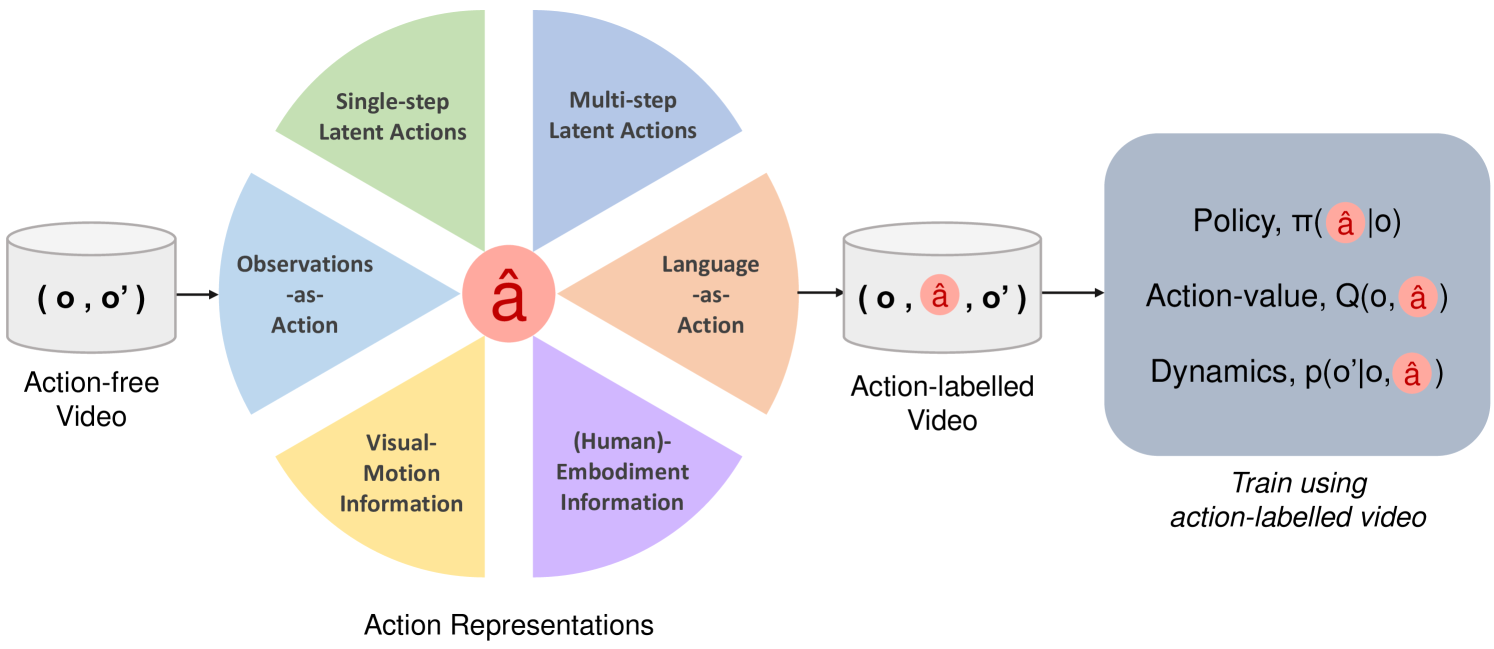
\includegraphics[width=1.0\linewidth]{./chapter5/media/RecoveringActionFepresentationsFromVideo_1}
	\caption[To label action-free videos, an Alternative action $\hat{a}$ can be derived from video data instead of the missing Action $a$]{To label action-free videos, an Alternative Action $\hat{a}$ can be derived from video data instead of the missing action $a$ \cite{McCarthy_2025}.}
	\label{fig:RecoveringActionFepresentationsFromVideo_1}
\end{figure}


The main challenges for transferring video-extracted knowledge to robotics are: 
\begin{enumerate}
    \item \textbf{Missing action labels}: Most video datasets do not contain explicit robot action annotations, which are required for learning robot control policies \cite{McCarthy_2025}.
    \item \textbf{Distribution shift}: There exists a significant domain gap between human/internet demonstrationvideos and robot execution. This includes differences in visual appearance, embodiment, dynamics, and behavior patterns, which can severely degrade the generalization of models trained on video data when applied to robotic tasks \cite{McCarthy_2025}.
\end{enumerate}

% ToDo: real world datasets with no robot labels
In many real-world video datasets, explicit robot action labels (e.g. joint velocities or torques) are not available.
% Problem. 
Raw video data provides only state transitions pairs $(o_t, o_{t+1})$, without access to the corresponding actions $a_t$. This makes it difficult to directly apply \ac{BC} or \ac{RL} methods, which typically require triplets of the form $(o_t, a_t, o_{t+1})$. Recovering such low-level actions directly from video is a challenging problem due to ambiguity and the lack of physical interaction information \cite{McCarthy_2025}. 
% Solution.
% To overcome this limitation, recent approaches introduce an Alternative Action Representation $\hat{a} \in \hat{A}$ within the alternative-action Space $\hat{A}$ so that transitions can be relabeled as $(o_t, \hat{a}_t, o_{t+1})$. 
To overcome this limitation, recent approaches introduce an \textbf{Alternative Action Representation} $\hat{a} \in \hat{A}$, which can be used to relabel action-free videos and enable video-to-robot transfer despite missing action labels and distribution shift, see Figure \ref{fig:RecoveringActionFepresentationsFromVideo_1}.

Formally, this induces a relabeling of video transitions as:
\begin{equation}
    (o_t, o_{t+1}) \;\rightarrow\; (o_t, \hat{a}_t, o_{t+1}), \quad \hat{a}_t \in \hat{A}.
\end{equation}

% To overcome this limitation, recent approaches introduce an Alternative Action Representation Space $\hat{A}$, where an alternative action $\hat{a} \in \hat{A}$ can be derived from video data, allowing transitions to be relabeled as $(o_t, \hat{a}_t, o_{t+1})$. 



% Video data provides state transition information in the form of $(o_t, o_{t+1})$ pairs, which can be used to derive alternative action representations $\hat{a}$ that capture the underlying behavior or intent of the observed transitions. By learning to predict $\hat{a}$ from video observations, the model can capture high-level behavioral patterns that are relevant for robotic control, even in the absence of direct action labels.

% To address these challenges, recent approaches introduce an alternative action representations $\hat{a} \in \hat{A}$ can be derived from video data, which can be used to label action-free videos and enable video-to-robot transfer despite missing action labels and distribution shift, see Figure \ref{fig:RecoveringActionFepresentationsFromVideo_1}. 

\subsection{What is an Alternative Action Representation?}
Formally, an alternative action representation is defined as
\begin{equation}
    \hat{a} \in \hat{A},
\end{equation}
where
$\hat{A}$ denotes an Alternative latent/abstract Action Representation Space. 
Instead of modeling actions as raw robot control signals, actions are encoded in a semantic feature space that captures high-level behavior such as grasping, moving, or pushing. In other words, $\hat{A}$ captures what actions \textit{mean}, rather than how it is executed at the motor level \cite{McCarthy_2025}.
% which are easier to infer from video, rather than the raw motor commands.
The key idea is that the action $\hat{a}$ serves as a proxy for the missing robot action labels $a$, allowing the model to learn from video data without requiring explicit action annotations. Later, $\hat{a}$ can be decoded or translated into the robot's actual action space if a mapping $f: A \to \hat{A}$ exist \cite{Wang2023MimicPlayLI, Wen2023AnypointTM, Du2023LearningUP}. Otherwise, they still provide valuable structure \cite{Bhateja2023RoboticOR, Schmidt2023LearningTA}. However it is also valid to define a $\hat{A}$ that requires labelled video (e.g., language captions) \cite{McCarthy_2025}.


\paragraph{Example} 
Consider a video of a human performing a pick-and-place task. The raw video data provides visual observations of the human's hand and the objects being manipulated, but does not include explicit robot action labels such as joint angles or end-effector velocities.
\begin{itemize}
    \item The \textbf{Video Encoder} extracts visual features (what is being done), see section~\ref{sec:VideoEncoder}.
    \item The \textbf{Action Embedding Space $\hat{A}$} captures \textit{abstract actions} such as \textit{reach}, \textit{grasp}, \textit{move up}.
    \item The \textbf{Policy $\pi_{alt}( \hat{a}_t | o_t, c), \quad \hat{a}_t \in \hat{A}$} predicts the next action \textit{in this latent action space} based on current visual observations and probably some additional context information $c$, see section~\ref{sec:AlternativeActionPolicy}.  
    \item Later, a \textbf{Decoder} $\pi(a_t \mid \hat{a}_t, o_t)$ or \textbf{Alignment Model $a_t = f_{align}(\hat{a}_t)$} maps these latent actions to the robot's real motor commands, see section~\ref{sec:AlternativeActionDecoder}.    
\end{itemize}



\paragraph{Why is $\hat{A}$ Useful?}

Working in the alternative action space $\hat{A}$ offers several advantages. 
\begin{itemize}
    \item \texttt{Bridging the Domain Gap:} $\hat{A}$ bridges the gap between human video data and robot control by focusing on action semantics rather than platform-specific motor commands \cite{McCarthy_2025}. 
    
    \item \texttt{Learning from Weak Labels:} $\hat{A}$ enables learning from raw or weakly labeled videos, since inferring high-level actions from video is easier than recovering low-level motor commands \cite{McCarthy_2025}.
    
    \item \texttt{Transferable Representations Across Embodiments:} $\hat{A}$ supports transfer across embodiments, because the same semantic action (e.g. ``open drawer'') can be instantiated by different robots with different kinematics \cite{McCarthy_2025}.
    % \item \texttt{Structured learning:} $\hat{A}$ provides a structured representation that can be used for learning policies, dynamics models, and value functions in a more data-efficient and generalizable way if $\hat{A}$ is well-structured, minimal, disentangled, and semantically consistent across embodiments.

    \item \texttt{Structured Learning:} A well-structured representation $\hat{A}$ that is minimal, disentangled, and semantically consistent across the state space encodes meaningful action information. This makes it easier to learn models that are predictive of both future observations (i.e. learning $p_{\text{alt}}(o_{t+1} \mid \hat{a}_t, o_t)$ instead of $p(o_{t+1} \mid o_t)$) and robot actions (i.e., learning $\pi(a_t \mid \hat{a}_t, o_t)$ instead of $\pi(a_t \mid o_t)$), leading to more data-efficient and generalizable policies, dynamics models, and value functions \cite{McCarthy_2025, Rybkin2018LearningWY, Bruce2024GenieGI}.
    The choice of abstraction level for $\hat{A}$ also plays a crucial role: 
    \begin{itemize}
        \item \textbf{Higher-level or longer-horizon representations} $\hat{A}$ (such as language-based actions) can benefit performance in complex, long-horizon tasks by providing broader context and intent. This is because they capture more abstract and semantically meaningful information that can guide decision-making over longer time scales, which is particularly beneficial for tasks that require planning and reasoning about future consequences \cite{McCarthy_2025}.
        \item \textbf{Lower-level or shorter-horizon representations} $\hat{A}$, which retain more fine-grained information, may be more effective for accurately reconstructing or decoding the original robot actions $a_t$ from the alternative actions $\hat{a}_t$ \cite{McCarthy_2025}.
    \end{itemize}
\end{itemize}
% It can improve data efficiency and generalization, since a well-structured alternative action space $\hat{A}$ that is minimal, disentangled, and semantically consistent allows both $\pi(\hat{a}_t \mid o_t)$ and $\pi(a_t \mid \hat{a}_t, o_t)$ to be learned more easily and with fewer samples.
% The desired characteristics are:


Once $\hat{A}$ is defined, the same representation can be used for example for:
\begin{itemize}
    \item policies $\pi_{\hat{A}}(\hat{a}_t \mid o_t)$ \cite{Schmidt2023LearningTA},
    \item dynamics models $p_{\hat{A}}(o_{t+1} \mid o_t, \hat{a}_t)$ \cite{Bruce2024GenieGI} or
    \item state-action value functions $Q_{\hat{A}}(o_t, \hat{a}_t)$ \cite{Bhateja2023RoboticOR},
\end{itemize}
which further encourages consistent and transferable action abstractions.


% Once $\hat{A}$ is defined, the same representation can be used not only for policies $\pi_{\hat{A}}(\hat{a}_t \mid o_t)$, but also for dynamics models $p(o_{t+1} \mid o_t, \hat{a}_t)$ or value functions $Q(o_t, \hat{a}_t)$, which further encourages consistent and transferable action abstractions.


%---------
% By learning to predict $\hat{a}$ from video observations, the model can capture high-level behavioral patterns that are relevant for robotic control, even in the absence of direct action labels.


% Action free Video data often lacks on explicit action labels for robotics. But it is difficult to recover these missing robot action labels from video data directly. 

% The Idea is to label the videos with an alternative Action $\hat{a} \in \hat{A}$ from an Alternative Representation Space $\hat{A}$, which should be easier than directly derive the specific robot action labels from video data.

% representations $\hat{a}$ from video data, which can serve as proxies for the missing action labels. 


% from $(o_t, o_{t+1})$ to $(o_t, \hat{a}_t, o_{t+1})$.

% To address this, we can derive alternative action representations $\hat{a}$ from video data, which serve as proxies for the missing action labels. These alternative representations can be obtained through various methods, such as:


% Goal: Recovering the missing action representations from video

\subsection{Categories of Alternative Action Representations}
\label{sec:CategoriesOfAlternativeActionRepresentations}


\begin{figure}[h]
	\centering
	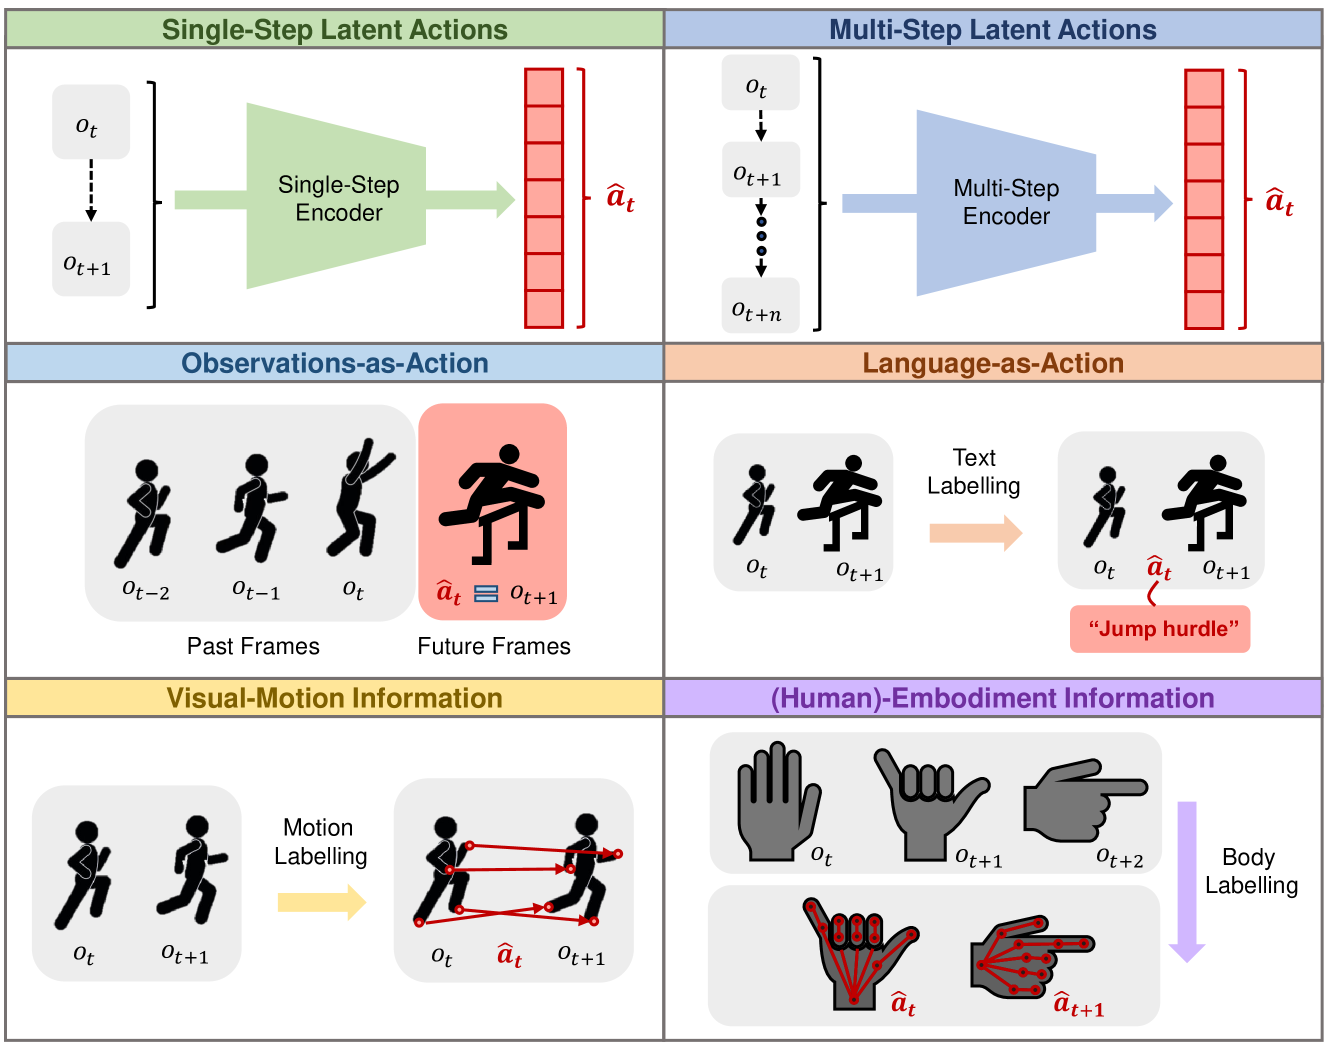
\includegraphics[width=1.0\linewidth]{./chapter5/media/RecoveringActionFepresentationsFromVideo_2}
	\caption[Categories of Alternative Action Representations that can be learned or obtained from video data.]{Categories of Alternative Action Representations that can be learned or obtained from video data
 \cite{McCarthy_2025}.}
	\label{fig:RecoveringActionFepresentationsFromVideo_2}
\end{figure}


Their exist different approaches to derive alternative action representations $\hat{a} \in \hat{A}$ from video data. These methods differ in how actions are represented and which information is extracted from visual observations \cite{McCarthy_2025}.







\paragraph{Single-step Latent Actions:}

These approaches learn latent actions in vectorized forms (=embedding) that describe the transition from one observation to the next \cite{McCarthy_2025}:
\begin{equation}
\hat{a}_t : o_t \rightarrow o_{t+1}
\end{equation}

\paragraph{Methods:}
The latent action $\hat{a}_t$ can be learned for example through:
\begin{itemize}
    \item \textbf{\ac{FDM}} $p(o_{t+1} \mid \hat{a}_t, o_t)$, which predict future observations from the current observation and latent actions \cite{Bruce2024GenieGI, Edwards2018ImitatingLP, Schmidt2023LearningTA, Ye2024LatentAP, Rybkin2018LearningWY}.
    \item \textbf{\ac{IDM}} $p^{-1}(\hat{a}_t \mid o_t, o_{t+1})$, which infer the latent action responsible for a transition \cite{Schmidt2023LearningTA, Bruce2024GenieGI}. 
    % To hinder the IDM from copying the entire observation $o_{t+1}$ into the latent action $\hat{a}_t$, the model is trained with some form of regularisation, such as a quantization bottleneck \cite{McCarthy_2025, Schmidt2023LearningTA, Bruce2024GenieGI}.
\end{itemize}

\paragraph{Limitations:}
\begin{itemize}
    \item Often capture all visual changes, not only agent actions \cite{McCarthy_2025}.
    \item May omit important non-visual information such as forces or contact dynamics \cite{McCarthy_2025}.
\end{itemize}








\paragraph{Multi-step Latent Actions:}

These methods encode behaviors across multiple time-steps in a single embedding:
\begin{equation}
\hat{a}_t : o_t \rightarrow o_{t+k}
\end{equation}

Instead of modeling individual actions, they capture higher-level behavioral patterns or latent plans \cite{McCarthy_2025}.
The key idea is to learn a compact latent representation of a \emph{skill} or \emph{sub-policy} that summarizes an entire sequence of actions. These representations are more abstract, goal orientated and can encode longer-horizon information, which may be beneficial for complex tasks \cite{RoseteBeas2022LatentPF, Cui2022FromPT, lynch2020learning}. 

For example these ``skill embeddings'' can capture structures such as ``reach the object'', ``move the arm to the target location'', or ``grasp and lift'', which can later be decoded into a full action sequence.


% Instead of modeling individual actions, they capture higher-level behavioral patterns or latent plans. These representations are more abstract, goal orientated and can encode longer-horizon information, which may be beneficial for complex tasks. 

% The key idea is that the model does not explicitly output every intermediate action, but instead learns a compact representation of a \emph{skill} or \emph{sub-policy} that executes a sequence of actions over time. These representations are more abstract, goal orientated and can encode longer-horizon information, which may be beneficial for complex tasks. 

% In this way, the representation captures higher-level structure such as ``reach the object'', ``move the arm to the target location'', or ``grasp and lift'', which can then be decoded into a full action sequence. This encourages the model to compress long action trajectories into a compact latent ``skill embedding'' that captures the essence of the behavior, rather than modeling every low-level action step.



\paragraph{Methods:}
\begin{itemize}
    \item \textbf{Variational Sequence Models:} These methods use \acp{VAE} to encode motion trajectories or sequences of observations into a latent variable $z$ that captures the underlying behavior. The VAE is trained to reconstruct the original trajectory from the latent representation \cite{Wang2023MimicPlayLI}.    
    % Variational auto-encoding of motion or trajectory representations 
    \item \textbf{Video-Language Contrastive Learning:} Aligns video segments with natural language descriptions of behaviors \cite{fan2022minedojo, Lifshitz2023STEVE1AG, Sontakke2023RoboCLIPOD}.
    \item \textbf{Supervised Contrastive Learning:} Pulls on a action-labeled dataset, videos with the same or similar action labels together in latent space, while pushing videos with different action labels apart \cite{ChaneSane2023LearningVP, Chen2021LearningGR}.
    \item \textbf{Self-Supervised Clustering Approaches:} Group similar motion patterns or trajectories into clusters without requiring labels, with each cluster representing a reusable skill or behavior primitive \cite{Xu2023XSkillCE}.
    \item \textbf{Further Approaches:} Presented in the works of Tomar et al. \cite{tomar2023video}, Pertsch et al. \cite{Pertsch2022CrossDomainTV}, and Cai et al. \cite{Cai2023GROOTLT}. 
    % include hierarchical sequence models and latent plan representations (e.g., Pertsch et al., Cai et al.), which explicitly model skills as temporally extended latent variables.
\end{itemize}

\paragraph{Limitations:}
\begin{itemize}
    % Quellen sollten passen
    \item Often produce abstract and long-horizon representations that may lose fine-grained control details and be harder to align with low-level robot actions \cite{kim2026hierarchical, liang2025clam}.
\end{itemize}






\paragraph{Observations-as-Actions:}

These approaches directly use (encoded) future observations as action representations:
\begin{equation}
    \hat{a}_t = o_{t+k}.
\end{equation}
Future observations provide information about the intended behavior or goal state \cite{McCarthy_2025}.

\paragraph{Methods:}
\begin{itemize}
    \item \textbf{Next-Observation-as-Action:} Uses the next observation $o_{t+1}$ as the $\hat{a}_t$ label and provides information regarding the action that should be taken \cite{Du2023LearningUP, Thomas2023PLEXMT, he2024large}.
    \item \textbf{Observations-as-Subgoals:} Uses future observations as intermediate goals to guide action selection \cite{Black2023ZeroShotRM, park2023hiql, Bhateja2023RoboticOR}. There exist different options to select the future observation that during training stage: 
    \begin{itemize}
        \item \textbf{Fixed Time Horizon:} Uses observations that are fixed $k$ time steps in advance \cite{Black2023ZeroShotRM, Du2023LearningUP}.
        \item \textbf{Random Time Horizon:} Uses observations that are a randomly sampled number of time steps in advance \cite{Bhateja2023RoboticOR}.
        \item \textbf{Key-Frame Selection:} Identifies critical states in a trajectory that can serve as action representations \cite{Pertsch2019KeyframingTF, liu2023learning}, see table \ref{tab:keyframes_pickplace}.
        
        \begin{table}[h]
            \centering
            \begin{tabular}{|c|l|l|}
                \hline
                \textbf{Time Step} & \textbf{Frame Description} & \textbf{Significance} \\
                \hline
                $t_0$ & Arm over table & Start \\
                $t_1$ & Arm approaches cup & Intermediate state \\
                $t_2$ & \textbf{Hand touches cup} & \checkmark\ Key-frame \\
                $t_3$ & Cup is lifted & Intermediate state \\
                $t_4$ & \textbf{Cup over target} & \checkmark\ Key-frame \\
                $t_5$ & Cup is placed & End \\
                \hline
            \end{tabular}
            \caption{Example Key-Frames in a Pick-and-Place Sequence}
            \label{tab:keyframes_pickplace}
        \end{table}
    \end{itemize}
\end{itemize}

\paragraph{Limitations:}
\begin{itemize}
    \item Future observations may not uniquely determine the underlying action \cite{A_hierarchical_representation_for_future_action_prediction}.
    \item High-dimensional visual observations can increase learning complexity \cite{A_hierarchical_representation_for_future_action_prediction, Losey2021LearningLA}.
\end{itemize}






% ToDo: Quelle 306, 7 evtl. hinzufügen
\paragraph{Language-as-Actions:}

Natural language descriptions can be used as high-level action representations for example by captioning video frames with language instructions that describe the observed behavior \cite{belkhale2024rt, shi2024yell, xiang2024pandora}:
\begin{equation}
\hat{a}_t = \texttt{"pick up the cube"}.
\end{equation}
Language-based actions provide semantic supervision and enable integration with \acp{LLM} \cite{Du2023VideoLP}, which can facilitate more complex reasoning and planning.

\paragraph{Methods:}
\begin{itemize}
    % ToDo: Quellen für diese beide Stichpunkte
    \item Video-to-Text Models \cite{McCarthy_2025}
    \item \acp{VLM} and variants of them \cite{McCarthy_2025}
\end{itemize}

\paragraph{Methods for Missing Language Captions:}
Video datasets may not always contain usable language captions. To address this, several methods can be used to generate or enhance captions for video data: 
\begin{itemize}
    % ToDo: Hier evtl. nochmal die Quellen nachprüfen
    % \item Language-captioned video datasets \cite{Grauman2021Ego4DAT}
    \item Process and enhance standard captions to generate more detailed action descriptions, for example by using \acp{LLM} or \acp{VLM} \cite{Mu2023EmbodiedGPTVP}.
    \item Usage of automated or semi-automated video captioning methods \cite{Mu2023EmbodiedGPTVP}
\end{itemize}


% ToDo: Quellen überprüfen und evtl. bessere suchen
\paragraph{Limitations:}
\begin{itemize}
    \item Language is often coarse and omits low-level control details \cite{McCarthy_2025}.
    \item Requires annotated or captioned video data \cite{McCarthy_2025}.
\end{itemize}






\paragraph{Visual Motion Information:}

These approaches define actions using visual motion cues extracted from video sequences \cite{McCarthy_2025}. The underlying assumption is that temporal changes in visual observations (motion patterns) contain implicit information about the actions responsible for observed state transitions. For example, the direction, magnitude, and trajectory of movement can provide information about the intended behavior, goal, or interaction dynamics \cite{yanokura2020understanding, Tokmakov17}.

\paragraph{Methods:}
\begin{itemize}
    \item \textbf{2D or 3D Point Trajectories:} Tracking objects or hands \cite{Wen2023AnypointTM, Yuan2024GeneralFA} via off-the-shelf point trackers \cite{karaev2024cotracker}
    \item \textbf{Optical Flow Predictions:} Capturing  how image regions move between consecutive video frames \cite{Ko2023LearningTA, xu2022gmflow}
    % \item Optical flow prediction, which captures how image regions move between consecutive video frames
    \item \textbf{Visual Action Arrows:} Representing movement direction and magnitude directly in the image \cite{Nasiriany2024PIVOTIV}
    \item \textbf{Structure-from-Motion Approaches:} Reconstructing 3D scene geometry and camera motion from video in order to recover information about underlying physical interactions \cite{Wang2023ManipulateBS, Yuan2021DMotionRV, Yang2023LearningIR}
\end{itemize}

\paragraph{Limitations:}
\begin{itemize}
    \item Motion estimates can be noisy or ambiguous \cite{booij2010efficient}.
    \item Visual motion does not always correspond directly to robot actions \cite{booij2010efficient}.
\end{itemize}




% ToDo: Quellen neu anordnen + überprüfen wo welche gebraucht wird.
% ToDo: Quelle 203 evtl. hinzufügen
\paragraph{(Human)-Embodiment Information:}

These approaches explicitly model human body structure and kinematics \cite{McCarthy_2025, Bharadhwaj2023TowardsGZ, Shaw2022VideoDexLD, Bahl2023AffordancesFH, Qin2022FromOH, Qin2021DexMVIL}. 
In contrast to generic motion-based methods, which focus on pixel or object movement, these approaches aim to represent the \emph{agent performing the action} using structured human pose information. 
Embodiment-specific information such as hand poses, affordances, or trajectories can provide useful cues about the intended actions and interactions in the video, which can be transferred to robotic embodiments \cite{rong2020frankmocap, Shan2020UnderstandingHH}.
For example, an alternative action representation can be defined as:
\begin{equation}
    \hat{a}_t = \text{hand pose at next time-step } t+1,
\end{equation}
which encodes the intended end-effector movement and can be associated with actions such as reaching, grasping, or manipulating objects. Animal embodiment data could also be useful \cite{peng2020learning}.
% which can be used to infer actions such as reaching, grasping, or manipulating objects.

\paragraph{Methods:}
\begin{itemize}
    \item \textbf{Human Pose Estimation:} Estimating full-body kinematics \cite{Bharadhwaj2023TowardsGZ}.
    \item \textbf{Hand Pose Estimation and Trajectory Tracking:} Estimating hand pose and tracking hand trajectories \cite{rong2020frankmocap, Shan2020UnderstandingHH}.
    \item \textbf{Affordance Prediction:} Predicting for example graspable regions, interaction points, and grasp trajectories \cite{Bahl2023AffordancesFH, Bharadhwaj2023TowardsGZ}.
    \item \textbf{Object- and Hand-Mask Conditioned Representations:} Focusing on regions of the video relevant for action understanding while ignoring irrelevant background information\cite{Bharadhwaj2023TowardsGZ}.
\end{itemize}

\paragraph{Limitations:}
\begin{itemize}
    \item Human embodiment is structurally different from robotic embodiments, limiting direct transferability.
    \item Accurate pose and hand tracking or estimation can be unreliable in cluttered or occluded scenes.
    \item Focuses on human-centric actions, which may not generalize to non-human interaction styles.
\end{itemize}




\paragraph{Inverse Dynamics Model (IDM) for Pseudo-Action Labels:}
It's not an alternative action representation in the strict sense, but it is a method to recover missing action labels from video data.
These methods train an inverse dynamics model on robot data and use it to infer pseudo-action labels for action-free (human) videos \cite{Baker2022VideoP, Torabi2018BehavioralCF, Schmeckpeper2020ReinforcementLW}, which can then be used for learning policies \cite{McCarthy_2025}:
\begin{equation}
p^{-1}(a_t \mid o_t, o_{t+1}).
\end{equation}

\paragraph{Limitations:}
\begin{itemize}
    \item Require action-labeled robot data for model training \cite{Baker2022VideoP, Torabi2018BehavioralCF, Schmeckpeper2020ReinforcementLW}.
    \item Domain shift between demonstration videos and robot execution \cite{Baker2022VideoP, Schmeckpeper2020ReinforcementLW, Kim2023GivingRA}.
\end{itemize}






